\chapter{Introduction}
\label{ch:intro}

% - General description of robotics;
% - General description of perception;
% - General description of localization.

Like many scientific terms that we encounter in our daily activities, \emph{robotics} describes a broad collection of technologies and stands at the intersection of key research directions. Motivated by practicality, disciplines that appear completely unrelated find themselves building upon advancements in other fields, diluting boundaries and joining forces to enable otherwise-impossible advancements.

What constitutes a \emph{robot}, then? In its inceptive use by Karel Čapek \cite{roberts_robotics_history_1999} in 1921, the word stemmed from the Slavic \emph{robota}, meaning ``servitude'' or ``forced work'', and referred to a human-like mechanical system working on factory assembly lines. This concept, however, dates from earlier centuries. Around 1495, Leonardo Da Vinci envisioned a mechanical knight controlled by a series of pulleys, that was able to perform simple movements \cite{taddei_leonardo_robots_2008}. Testifying to the industrial revolution and the computational breakthroughs of the last few decades, modern-day humanoid robots can perform acrobatics \cite{bostondynamics_backflips_2023}, interact with humans in constrained scenarios \cite{humanoids_hospital} \cite{humanoid_school} \cite{humanoid_school2} and even replicate human facial expressions \cite{humanoid_facial}. Still, a device ought not necessarily appear human-like in order for it to be labeled as a robot. Autonomous vacuum cleaners, space rovers or crop-monitoring drones fall under the same category. At this stage, a complete taxonomy would have to address dozens of physical (size, shape, mobility, locomotion system, etc.) and non-physical (autonomy, perception abilities, use-case, etc.) characteristics, and none of these would independently convey the meaning that we intuitively associate to the notion of \emph{robot}. Without assessing whether an exhaustive, generic definition is even possible, we can synthesize the above by affirming that a \emph{robot} is an artificial system that performs one or more tasks and is able to evaluate its state or gather information from its environment.

\section{Robotic perception}

This formulation highlights two essential aspects of a robotic agent \reffig{robot-env}: actuation, seen as some form of dynamic physical ability, allowing the agent to enact the desired behavior, and perception, the ability to observe changes in the environment.

% Certainly, this  obfuscates several other key elements, such as control mechanisms, information management or a reasoning model, but it emphasizes the importance of perception as a vital link with the physical world. Additionally, this closely resembles the behavior model of humans, where sensing also plays a critical role.

\begin{figure}[H]
    \centering
    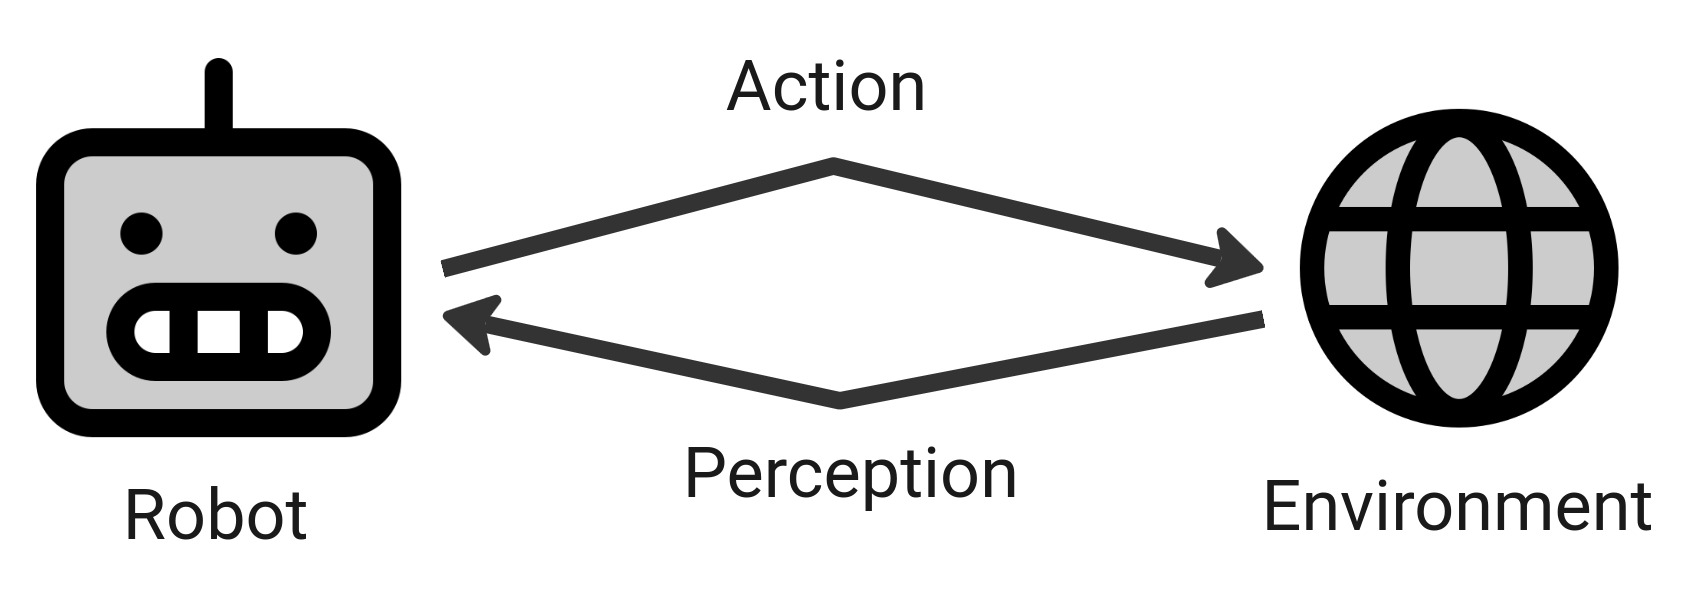
\includegraphics[width=0.7\linewidth]{robot-env.jpg}
    \caption[Perception in the Robot-Environment exchange]{A simplified interpretation of the robotics paradigm. The interaction between an agent and its environment can be seen as a two-way flow: the agent alters the environment through its actions, and uses perception to observe it.}
    \label{fig:robot-env}
\end{figure}

% Just as the human senses span multiple stimulus modalities, so does artificial perception, through the use of different types of sensors. An initial categorization differentiates between proprioceptive and exteroceptive sensors. The first type refers to sensors that provide information about the internal state of the system (virtually independent from the environment), while the second type consists of sensors that collect data about the world. Another division classifies sensors as active (emitting some form of energy in order to obtain a reading) or passive (which simply react to external stimuli).

Sensing modalities have largely different contributions to the perception mechanism. To this extent, the phrase \emph{visual dominance} was introduced by F. Colavita \cite{colavita1974human}, whose study demonstrated that humans focus more on the visual component when presented with an audiovisual stimulus, and following research has strongly confirmed this tendency \cite{Hutmacher2019} \cite{hecht2009sensory}. Unsurprisingly, a similar pattern is emerging in the case of robots, thanks to the reduced cost, familiarity and wide availability of cameras. In many situations, visual stimuli provide most of the necessary information, and this has motivated the development of various image processing algorithms.

Technological innovation in the last century has lead to the situation in which artificial sensors surpass humans in both the range of signals that are perceived, as well as the accuracy of the measurements. A relevant example is the class of \acrfull{lidar} sensors which retrieve three-dimensional information about the environment at a very high frequency and with rather negligible measurement errors, in the form of \emph{\glspl{pointcloud}}. Among many applications, this type of sensors can be used to construct virtual representations of a specific environment, enabling engineers to experiment with a realistic model, evaluate construction progress or validate a finished project.

\section{Problem definition}

The current work addresses a common and well-known problem in the area of \gls{fieldrob}, namely \acrfull{slam}, and combines the practicality of an industrial solution with a perception-based approach.

\begin{figure}
    \centering
    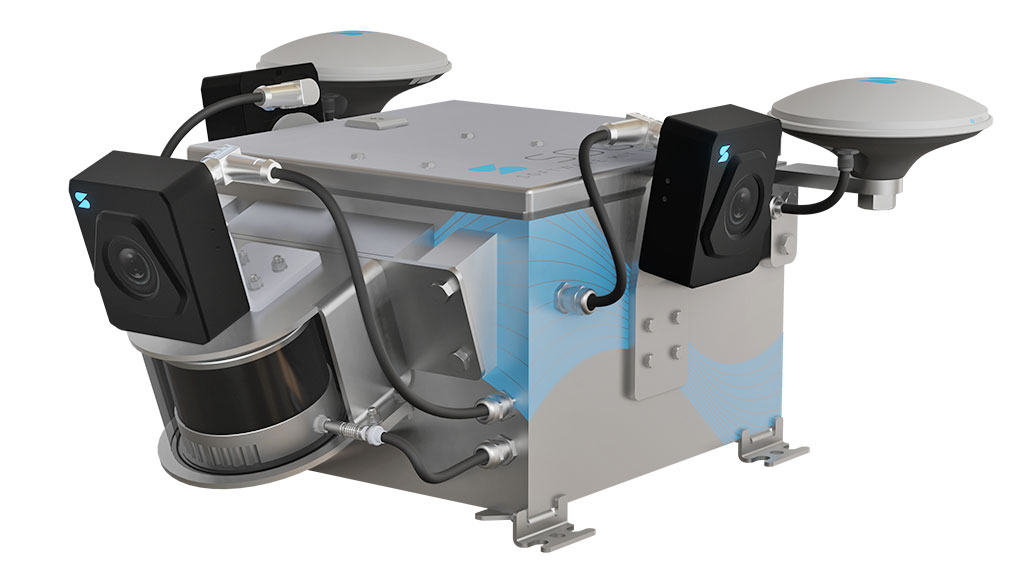
\includegraphics[width=0.6\linewidth]{images/sdx-compact.jpg}
    \caption[SDX-Compact]{The SDX-Compact manufactured by Sodex Innovations GmbH. The set of sensors consists of a 3D LiDAR scanner, three RGB cameras and a high-accuracy positioning system. Image source: \href{https://fieldwork.ch/de/produkte/geopositioning/mobile-datenerfassung/sdx-compact}{Fieldwork}}
    \label{fig:sdx-compact}
\end{figure}

SDX-Compact \reffig{sdx-compact} is the main product of Sodex Innovations GmbH, consisting of multiple sensors that collect spatial and visual data. This module can be easily mounted on an arbitrary vehicle in order to expand its perception capabilities and convert it into a \gls{surveying} device. While the vehicle is moving, the LiDAR sensor captures 3D scans of the surroundings, as well as related metadata (timestamps, localization information, signal intensity etc.). Because the rig includes a high-accuracy \acrfull{ins}, the localization and orientation data can be used to join the collected point clouds and create a global 3D map of the traversed space.

Nonetheless, this suffers from two main limitations:

\begin{compactitem}
    \item Reliance on unstable signal: internally, the  depends on information from a \acrfull{gnss} receiver, which is limited to outdoor spaces and whose availability varies depending on weather conditions and surroundings (e.g. thick vegetation, tall buildings, bridges). 
    \item Unsatisfactory accuracy: when merging point cloud data, positioning or localization errors introduce inconsistencies in the final 3D model, which hinders precise planning and construction.
\end{compactitem}

Our work aims to address these limitations by introducing a component that utilizes the information collected by the LiDAR sensor in conjunction with the existing data. Three research questions have been formulated to guide this process:

\begin{compactenum}
    \item What metrics exist for measuring the accuracy of point cloud \gls{registration}? In this context, registration refers to placing a pair of related point sets in a common reference frame.

    \item Can methods that use only visual information achieve higher quality point cloud registration (3D mapping) than merging based on \acrfull{rtk}? Usually, GNSS systems provide meter-level accuracy. In the current scenario, however, the system is corrected using Real-Time Kinematics, such that the expected error is at centimeter-level.

    \item To what extent is LiDAR-based \gls{odometry} an alternative to GNSS localization? Previous research indicates that the spatial information present in 3D point clouds could be used to compute the relative displacement between consecutive scans, resulting in the ability to estimate odometry (an essential component of robotic localization) without dedicated sensors such as wheel encoders or accelerometers.
\end{compactenum}

The main contribution of the project consists of developing an original framework for localization and mapping based on data collected with an industrial sensor rig. The results are more generic than if a particular physical robotic system were involved, and thus are relevant for virtually any robotic application with a similar setup.

The following chapters of this document will cover related research directions and efforts that our work builds upon \refch{review}, a detailed description of the components and algorithms involved in developing the project \refch{methodology}, an evaluation of the method based on its results \refch{results}, as well as a series of conclusions that were drawn from the overall process \refch{conclusion}.

% evaluation to enable future use
% document structure



% research questions
% motivation/justification
% scope, limitations
